\section{Abstract Interpretation}\label{sec:abstrint}

Abstract interpretation is among the most well known methods of static
analysis of programs. First introduced by Patrick and Radhia Cousot
in~\cite{patrickradhia:one, patrickradhia:two} and consists in a
sound-by-construction method to infer program properties given a model
of their behavior. The general idea is that we can approximate the
semantics of a program with monotonic functions over ordered sets
(usually \emph{complete lattices}). To do so we usually first
introduce \emph{Abstract Domains} that capture some essential aspect
of program execution while ignoring the details of the computation,
which would make the analysis computationally infeasible.  This
analysis however carries the issue of completeness, which is closely
related to the issue of choosing the best abstract domain to decide
program correctness without raising false alarms. Achieving
completeness in analysis is often desirable, but it can lead to the
problem of undecidability. This means that even though we strive for
the most accurate analysis of a program, such as through its
interpreter, we can't guarantee that the process will always
terminate.  The technique per-se is a concept which is around since
the '70s, hence an extensive amount of literature has been
produced. For a brief history of the technique,
see~\cite{ranzato:history}.

The main source of this chapter comes from the notes on abstract
interpretation by Prof.\ Miné~\cite{mine:course}.

\subsection{General concepts}\label{subsec:abstrgeneral}

Abstract interpretation heavily relies on order theory, which we
introduced in Section~\ref{sec:ordertheory}, and builds on top of
it. The core idea is that we use an \emph{abstract domain} as an
approximation of the \emph{concrete domain}, in such a way that
abstract computations are \emph{sound} with respect to the concrete
ones. The minimal structure that we will require both in the abstract
and the concrete domains is a partial order that models the amount of
information each instruction carries with respect to the program
execution. Thus, the concrete domain is a partially ordered set
\(\tuple{C, \leq}\) (e.g.\ integers powersets) and the abstract domain
is another partially ordered set \(\tuple{A, \sqsubseteq}\) (e.g.\
intervals). The minimal amount of connection between these two worlds
is a \emph{concretization} functions
\begin{definition}[Concretization]
  A concretization function
  \(\gamma : \tuple{A , \sqsubseteq} \to \tuple{C, \leq}\) is a
  \emph{monotonic} function, i.e.
  \begin{equation*}
    \forall a,a' \in A \quad a \sqsubseteq a' \Rightarrow \gamma(a) \leq \gamma(a')
  \end{equation*}
\end{definition}

Trough concretization we have a first notion of \emph{soundness}

\begin{definition}[Soundness]
  \(a \in A\) is a \emph{sound} abstraction of \(c\in C\) iff
  \(c \leq \gamma(a)\).
\end{definition}

While monotonic concretizations are sufficient to reason about
soundness, more structure is useful to design a sound and
\emph{accurate} analyzer. The standard abstract interpretation
framework from~\cite{patrickradhia:one} also assumes the existence of
some monotonic \emph{abstraction function}
\({\abstr : \tuple{C, \leq} \to \tuple{A, \sqsubseteq}}\), such that
\(\tuple{\abstr, C, A, \concr}\) forms a Galois connection:

\begin{definition}[Galois connection]
  Given two partially ordered sets
  \(\tuple{C, \leq}, \tuple{A, \sqsubseteq}\), the tuple
  \(\tuple{\abstr, C, A, \concr}\) is a Galois connection if
  \begin{itemize}
  \item \(A,C\) are complete lattices;
  \item \(\abstr : \tuple{C, \leq} \to \tuple{A, \sqsubseteq}\) and
    \(\concr : \tuple{A, \sqsubseteq} \to \tuple{C, \leq}\) are monotonic;
  \item for all \(a\in A, c\in C\), \(c \leq \concr(a) \iff \abstr(c) \sqsubseteq a\).
  \end{itemize}

  Figure~\ref{fig:galois} is a visualization of the notion of Galois
  connection.
\end{definition}

\begin{figure}
  \centering
  \usetikzlibrary {arrows.meta}
  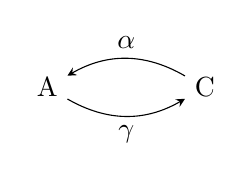
\begin{tikzpicture}[->, >=stealth]
    % Nodes
    \node (A) at (0,0) {A};
    \node (C) at (2,0) {C};
    
    % Arrows
    \path
    (C) edge[bend right=30] node[above]{$\alpha$} (A)
    (A) edge[bend right=30] node[below]{$\gamma$} (C);
  \end{tikzpicture}
  \caption{Galois connection between an abstract domain \(A\) and a
    concrete domain \(C\)}\label{fig:galois}
\end{figure}

Galois connections carry with them some well known properties, that
are useful to state best correct approximations (bca) and to prove the
soundness by construction of the analyzer:

\begin{theorem}[Galois connection properties]\label{th:galoisprop}
  Given a Galois connection \(\tuple{\abstr, C, A, \concr}\) we have:
  \begin{enumerate}
  \item \(\concr \circ \abstr \circ \concr = \concr\) and
    \(\abstr \circ \concr \circ \abstr = \abstr\);
  \item \(\abstr \circ \concr\) and \(\concr \circ \abstr\) are
    idempotent;
  \item \(\forall c \in C\)
    \(\abstr(c) = \sqcap \{a \mid c \leq \concr(a)\}\);
  \item \(\forall a \in A\)
    \(\concr(a) = \vee \{ c \mid \abstr(c) \sqsubseteq a \}\);
  \item \(\abstr\) maps concrete lubs to abstract lubs:
    \begin{equation*}
      \forall X \subseteq C \quad \exists \vee X \Rightarrow \abstr(\vee X) = \sqcup \{\abstr(x) \mid x \in X\}
    \end{equation*}
  \item \(\concr\) maps abstract lubs to concrete lubs:
    \begin{equation*}
      \forall X \subseteq A \quad \exists \sqcap X \Rightarrow \concr(\sqcap X) = \wedge \{\concr(x) \mid x \in X\}
    \end{equation*}
  \end{enumerate}
\end{theorem}

Theorem~\ref{th:galoisprop} states two important properties of Galois
connections: \emph{soundness} and \emph{optimality}. Additionally, from
the theorem we can derive the following corollary:

\begin{corollary}[Best abstraction]\label{co:bestabstr}
  If we have a Galois connection \(\tuple{\abstr, C, A, \concr}\),
  then \(\forall c \in C, \abstr(c)\) is the \emph{best abstraction}
  of \(c\), i.e., the smallest abstract element which is a sound
  abstraction of \(c\).
\end{corollary}

In general we saw that for a Galois connection \(\concr \circ \abstr\)
is idempotent, and generally not the identity function, as abstracting
looses precision. Concertizing however, should not loose precision, so
we could expect \(\abstr \circ \concr\) to be the identity
function. When this is the case, we have a \emph{Galois insertion}:

\begin{definition}[Galois Insertion]
  A Galois connection \(\tuple{\abstr, C, A, \concr}\) is a
  \emph{Galois insertion} if one of the following, equivalent
  properties hold:
  \begin{enumerate}
  \item \(\abstr\) is surjective: \(\forall a \in A\)
    \(\exists c \in C \mid \abstr(c) = a\);
  \item \(\concr\) is injective: \(\forall a, a'\in A\)
    \(\concr(a) = \concr(a') \Rightarrow a = a'\);
  \item \(\abstr \circ \concr\) is the identity function.
  \end{enumerate}
\end{definition}

In this context we also need a way of ensuring abstract operations are
sound (and occasionally) correct. Even by only using the
concretization map and no Galois connection, the notion of sound and
correct abstraction carries naturally from domain elements to domain
operators:

\begin{definition}[Sound and correct operator abstraction]
  Let \(\concr : \tuple{A \sqsubseteq} \to \tuple{C, \leq}\) be a
  concretization map from an abstract domain
  \(\tuple{A, \sqsubseteq}\) to a concrete domain \(\tuple{C, \leq}\),
  \(f : C \to C\) be a concrete operator and \(g : A \to A\) an
  abstract operator.
  \begin{enumerate}
  \item \(g\) is a \emph{sound abstraction} of \(f\) if
    \(\forall a \in A \quad f(\concr(a)) \leq \concr(g(a))\);
  \item \(g\) is a \emph{correct abstraction} of \(f\) if
    \(f \circ \concr = \concr \circ g\).
  \end{enumerate}
\end{definition}

Notice that a correct abstraction is always sound.  Another remarkable
thing of Galois connections, is that along with this notion we can
introduce the notion of \emph{Best correct approximation}:

\begin{definition}[Best correct approximation (bca)]
  Given a Galois connection \(\tuple{\abstr, C, A, \concr}\) and a
  concrete operator \(f : C \to C\), the \emph{best abstraction} of
  \(f\) is given by \(\abstr \conc f \conc \concr\).
\end{definition}

\todo[inline]{fixpoint calculation problems}

In order to solve the convergence problem in abstract
domains,~\cite{patrickradhia:one} introduced a specific binary
operator, the widening operator \(\widen\):

\begin{definition}[Widening operator]
  A binary operator \(\widen : A \times X \to A\) is a \emph{widening
    operator} in an abstract domain \(\tuple{A, \sqsubseteq}\) if
  \begin{enumerate}
  \item it computes upper bounds:
    \begin{equation*}
      \forall x, y \in A \quad x \sqsubseteq x \widen y \; \land \; y \sqsubseteq x \widen y;
    \end{equation*}
  \item it enforces convergence: for any sequence \(\{y^i\}_{i\in\n}\)
    in \(A\), the sequence \(\{x^i\}_{i\in\n}\) computed as
    \begin{align*}
      x^0 & \defin y^0 \\
      x^{i+1} & \defin x^i \widen y^{i+1}
    \end{align*}
    stabilizes in finite time: \(\exists k \geq 0 \mid x^{k+1} = x^k\).
  \end{enumerate}
\end{definition}

the latter definition allows us to observe several things:
\begin{itemize}
\item the first point allows to construct increasing sequences by
  iterating abstract operations that are not necessarily monotonic, and
  the result of \(x \widen y\) is a sound approximation of the
  concrete join \(\concr(a) \vee \concr(b)\);
\item the second point ensures that all increasing sequences with
  widening are finite: even if the abstract domain has infinite
  strictly increasing chains.
\end{itemize}

A naïve widening operator that can be used in any abstract domain
containing a top element \(\top\) could be the following:

\begin{example}[Naïve widening]
  \begin{equation*}
    x \widen y \defin \begin{cases}
      x & \text{if } y \sqsubseteq x \\
      \top & \text{otherwise}
    \end{cases}
  \end{equation*}
\end{example}

which we can see respects all the properties of the widening
definition and ensures convergence of strictly increasing chains.
Notice however that in doing so we \emph{loose} precision. I can
happen however that we can retrieve some of the lost precision by
looking at the syntax of the program we are considering. We can do
this by using the \emph{narrowing} operator:

\begin{definition}[Narrowing]
  A binary operator \(\narrowi : A \times A \to A\) is a
  \emph{narrowing operator} in an abstract domain
  \(\tuple{A, \sqsubseteq}\) if
  \begin{enumerate}
  \item it computes lower bounds:
    \begin{equation*}
      \forall x, y \in A \quad x \sqcup y \sqsubseteq x \narrowi y \sqsubseteq x;
    \end{equation*}
  \item it enforces convergence: for any sequence \(\{y^i\}_{i\in\n}\)
    in \(A\), the sequence \(\{z^i\}_{i\in\n}\) computed as
    \begin{align*}
      z^0 & \defin y^0 \\
      z^{i+1} & \defin z^i \narrowi y^{i+1}
    \end{align*}
    stabilizes in finite time: \(\exists k \geq 0 \mid x^{k+1} = x^k\).
  \end{enumerate}
\end{definition}

Where the first point states that \(\narrowi\) refines its left
argument while bringing a sound approximation, and the second point
enforces termination.
